\documentclass[12pt, a4paper, oneside]{article}
\usepackage{amsmath, amsthm, amssymb, bm, graphicx, hyperref, mathrsfs,color}

\begin{document}

%\maketitle
\begin{center}
	\rule{\textwidth}{1pt}\par
	\vspace{5mm}
	{\large\scshape UM-SJTU Joint Institute}\\[\baselineskip]
	{\large\scshape Physics Laboratory}\\
	(Vp241)
	\rule{\textwidth}{1pt}\par
	\vspace{4cm}
	{\large\scshape Laboratory Report}\\[\baselineskip]
	{\large\scshape Excercise 1}\\[\baselineskip]
	{\large\scshape Basic Characteristics of Magnetic Materials}\\[\baselineskip]
\end{center}
\vspace{7cm}

\begin{tabular}{lll}
	Name:Kaixuan Wang & ID:523370910219 & Group:11 \\
	Date: {\today}    &                 &         \\
\end{tabular}


\rightline{\footnotesize[rev4.1]}
\pagebreak

\section{Introduction}
% \textcolor{blue}{This part should include a brief description of the experiment: its objectives, underlying physical model and phenomena, and equations that you will use in
% 	your calculations. It may be a bit longer than that below, but you should not simply copy the lab manual or quote long passages from textbooks.}
\indent

The goal of this exercise is to study the shape of the magnetic hysteresis loop and the
magnetization curve, and understand how to use these characteristics to discuss properties
of ferromagnetic materials. For calculation, the magnetization curve and the magnetic hysteresis loop will
be visualized on the oscilloscope. 

\section{Experimental setup}
\indent

\subsection{Conceptual Questions}
\indent

Before going on with the experiment, we first answer the following concepts: 

\begin{itemize}
    \item \textbf{Magnetic Dipole Moment}: It is a vector quantity that represents the strength and orientation of a magnetic source, such as a current loop or a magnet. It measures the tendency of a system to align with a magnetic field.

    \item \textbf{Magnetization}: It refers to the degree to which a material becomes magnetized when exposed to a magnetic field. It is defined as the magnetic moment per unit volume of a material.

    \item \textbf{Antiferromagnetic vs. Ferromagnetic Ordering}:
    \begin{itemize}
        \item \textbf{Antiferromagnetic Ordering}: In this type of magnetic ordering, adjacent atomic spins align in opposite directions, resulting in no net magnetization.
        \item \textbf{Ferromagnetic Ordering}: In ferromagnetic materials, atomic spins align parallel to each other, leading to a strong net magnetization even without an external magnetic field.
    \end{itemize}

    \item \textbf{Hysteresis Loop}: A curve showing the relationship between the magnetic field applied to a ferromagnetic material and its resulting magnetization. It demonstrates the material's magnetic memory, showing how magnetization lags behind changes in the applied field.

    \item \textbf{Curie Temperature}: The temperature above which a ferromagnetic material loses its permanent magnetic properties and becomes paramagnetic, meaning that thermal energy disrupts the alignment of magnetic moments.
\end{itemize}

\subsection{Equipments used in the experiment}
\indent

Devices used in this experiment include the following: a signal generator, an oscilloscope, a digital multimeter, 
a voltage/current source, a wiring block, a capacitor, and two resistors with resistance value of 10$\Omega$ and 1000$\Omega$. 

\subsection{Measurements used in the experiment}
\indent

There is only one measurement to do in this lab: the Magnetic Hysteresis Loop Measurement. To carry out the measurement, we build a circuit shown in the Figure \ref{fig1}:

\begin{figure}[htbp]
	\centering
	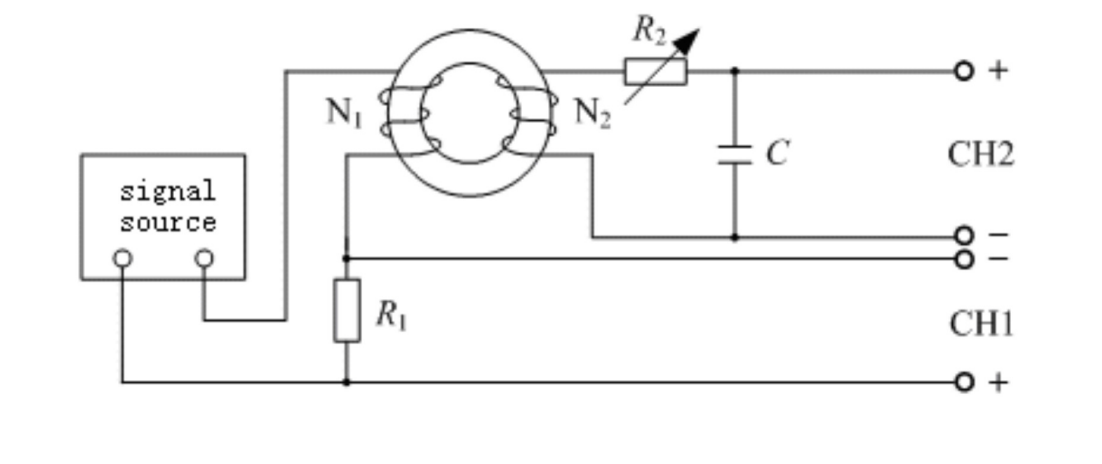
\includegraphics[width=0.9\textwidth]{fig1.png}
	\caption{Circuit setup}
	\label{fig1}
\end{figure}

Before measuring the desired $U_C$ and $U_R$, we need to measure the two values of resistance and capacity using the multimeter. After measuring, take
down the values for further calculations.  

The voltage of the capacitor and the 10$\Omega$ resistor is displayed on the oscilloscope for further measurement. After adjusting the amplitude and frequency of the output signal, we take 18 points 
on the loop as 18 groups of data to record. Using these groups of data, we calculate 18 groups of value of $H$ and $B$ using the following equation:

\begin{equation}
	H=\frac{N_1}{R_1L}U_{R_1}
	\label{eq1}
\end{equation}

\begin{equation}
	B=-\frac{R_2C}{N_2S}U_C
	\label{eq2}
\end{equation}

Finally using the data of $H$ and $B$ we plot the graph of H-B curve and find $\pm B_s$, $\pm B_r$, $\pm H_s$ and $\pm H_c$.

\section{Measurements and Results}
\subsection{Magnetic Hysteresis Loop Measurement}
\indent

Using the measurement method described above, we obtain the following data table: 

\begin{figure}[htbp]
	\centering
	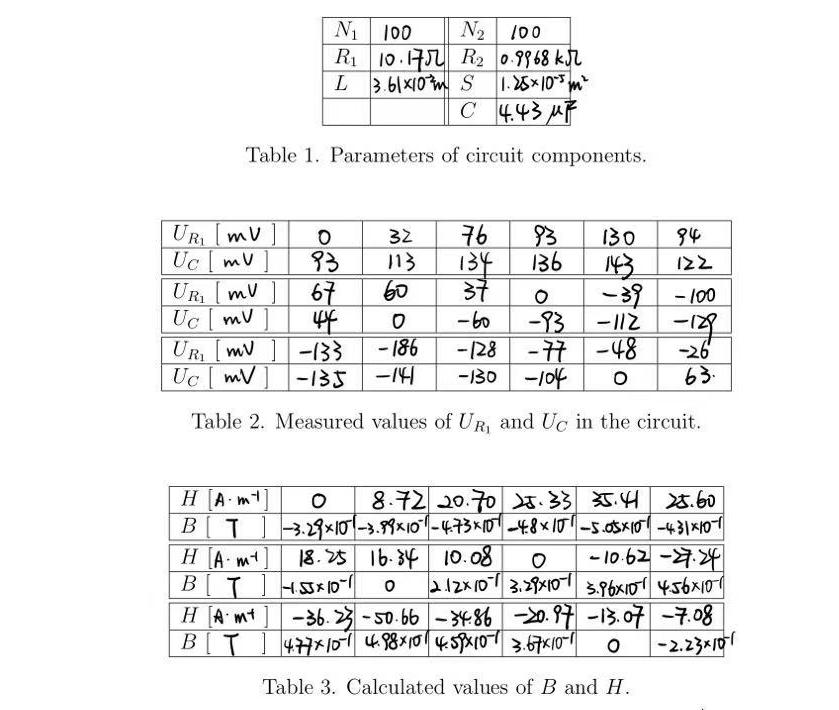
\includegraphics[width=0.9\textwidth]{fig2.png}
	\caption{Data tables of the experiment}
	\label{fig2}
\end{figure}

Table 1 is the data table of some essential parameters we will be using in the later calculation. In table 2 are the original groups of data obtained
from the oscilloscope. Table three contains the calculated $H$ and $B$ using the equations \ref{eq1} and \ref{eq2}. 

\section{Conclusions and discussion}
\indent

\subsection{H-B Curve and desired values of data}
\indent

In this experiment, we will plot the graph of H-B curve based on the data groups obtained above. We will use python to do the plotting. The 
curve is shown below:

\begin{figure}[htbp]
	\centering
	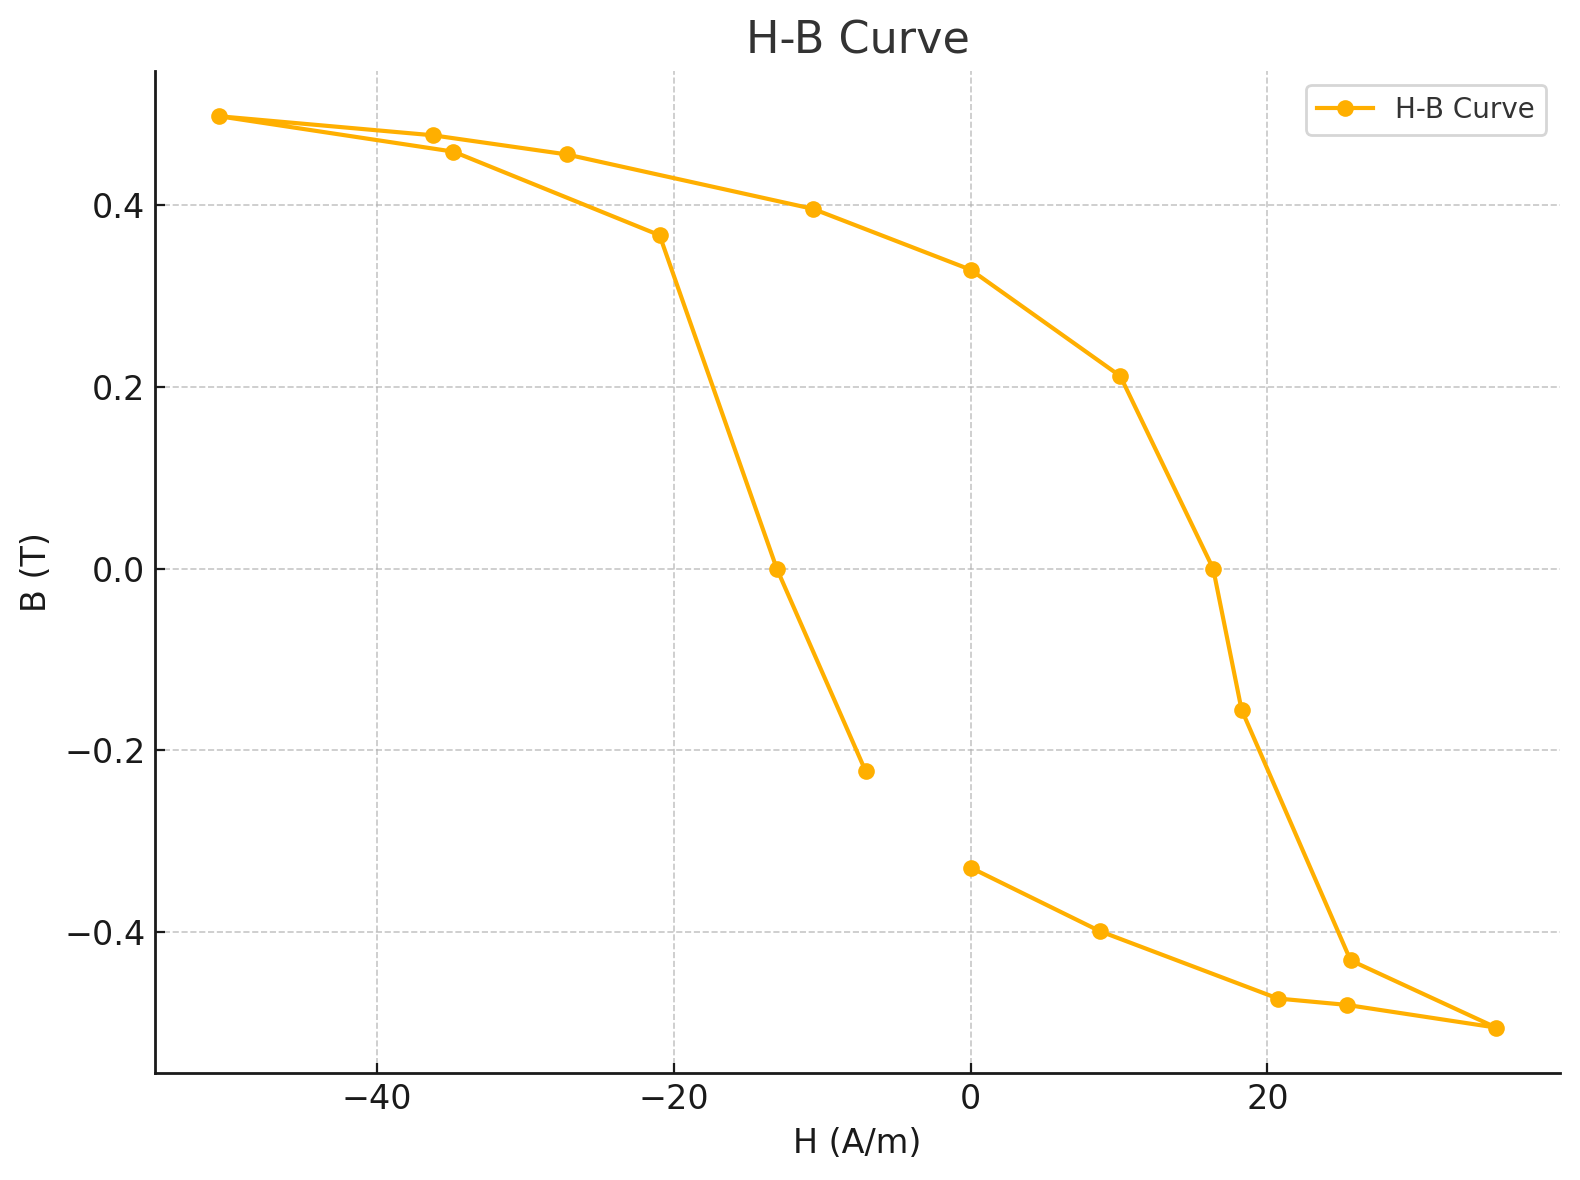
\includegraphics[width=0.9\textwidth]{fig3.png}
	\caption{H-B curve}
	\label{fig3}
\end{figure}

From the graph we can find the values of $\pm B_s$, $\pm B_r$, $\pm H_s$ and $\pm H_c$ as following:
\begin{itemize}
    \item $\pm B_s$: $B_s^+ = 0.498 \, \text{T}$, $B_s^- = -0.505 \, \text{T}$
    \item $\pm B_r$: $B_r^+ = 0.329 \, \text{T}$, $B_r^- = -0.329 \, \text{T}$
    \item $\pm H_s$: $H_s^+ = 35.41 \, \text{A/m}$, $H_s^- = -50.66 \, \text{A/m}$
    \item $\pm H_c$: $H_c^+ = 16.34 \, \text{A/m}$, $H_c^- = -13.07 \, \text{A/m}$
\end{itemize}

\subsection{Discussion}
\indent

From the final output of rthe graph we may see some steps that can be further improved. The shape of the curve is similar to what we desire as 
a Magnetic Hysteresis Loop, but it is still not symmetrical enough (or say, not smooth enough). This indicates some probable inaccuracy
in calculation or the process of data obtaining. One ideal solution to this problem is to take more groups of data to make up for the loss of accuracy.
Also, the whole measurement process is done manully choosing data points, which may also make the distribution of data not even or average. It would 
be great if there are some automatic programs that help choose data points at higher accuracy for better data distribution. 

\section{Works cited}
Department of Physics, Shanghai Jiaotong University, Exercise 1 (Basic Characteristics of Magnetic Materials) - lab manual [rev. 2.4], 2024\\
Python Software Foundation. (2020). Python Language Reference, version 3.9. Available at http://www.python.org\\
\\
All the figures displayed in the article (excluding the appendix) are given using Python 3.9.
\pagebreak
\appendix
\section{Datasheet}

\begin{figure}[htbp]
	\centering
	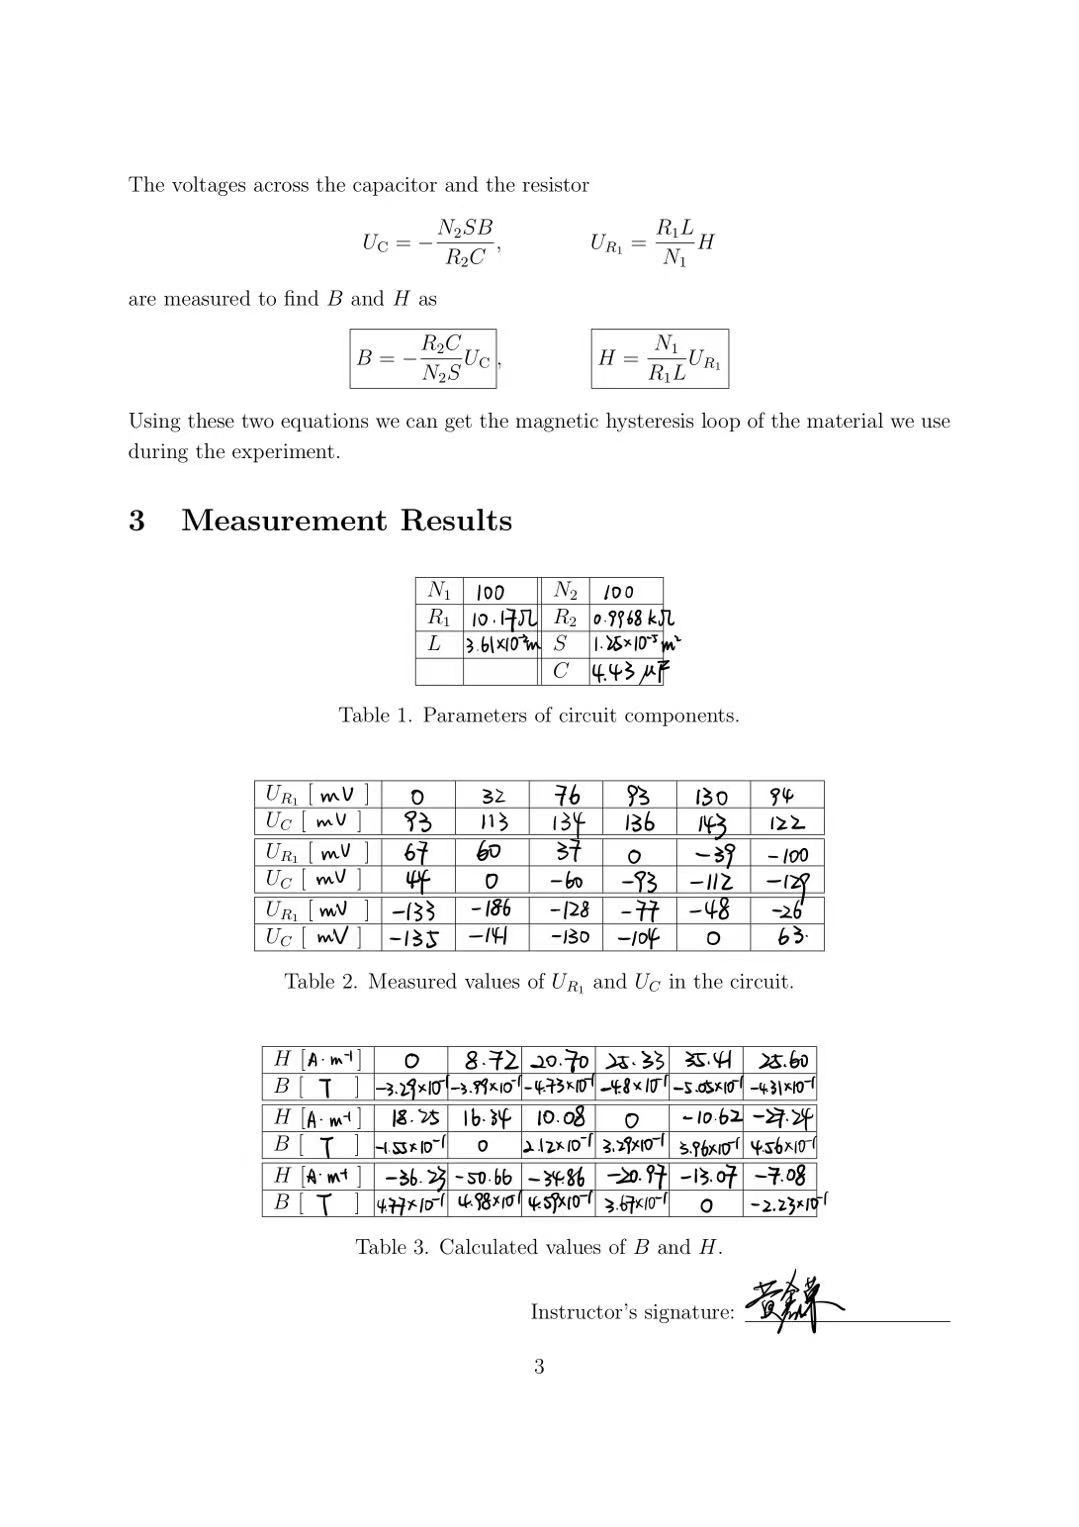
\includegraphics[width=0.75\textwidth]{D1.jpg}
	\caption{Datasheet 1}
\end{figure}


%\textcolor{blue}{Please remember to attach the original data sheet signed by your instructor.}
\end{document}